\documentclass[letterpaper,12pt,fleqn]{article}
\usepackage{matharticle}
\usepackage{tikz}
\usepackage{pgfplots}
\pgfplotsset{compat=1.14}
\pagestyle{plain}
\begin{document}

\begin{center}
  \large
  Math-19 Section 1

  \Large
  Homework \#4 Solutions
\end{center}

\subsection*{Problems}

\begin{enumerate}
\item Use the graph of $y=f(x)$ to answer the following questions:

  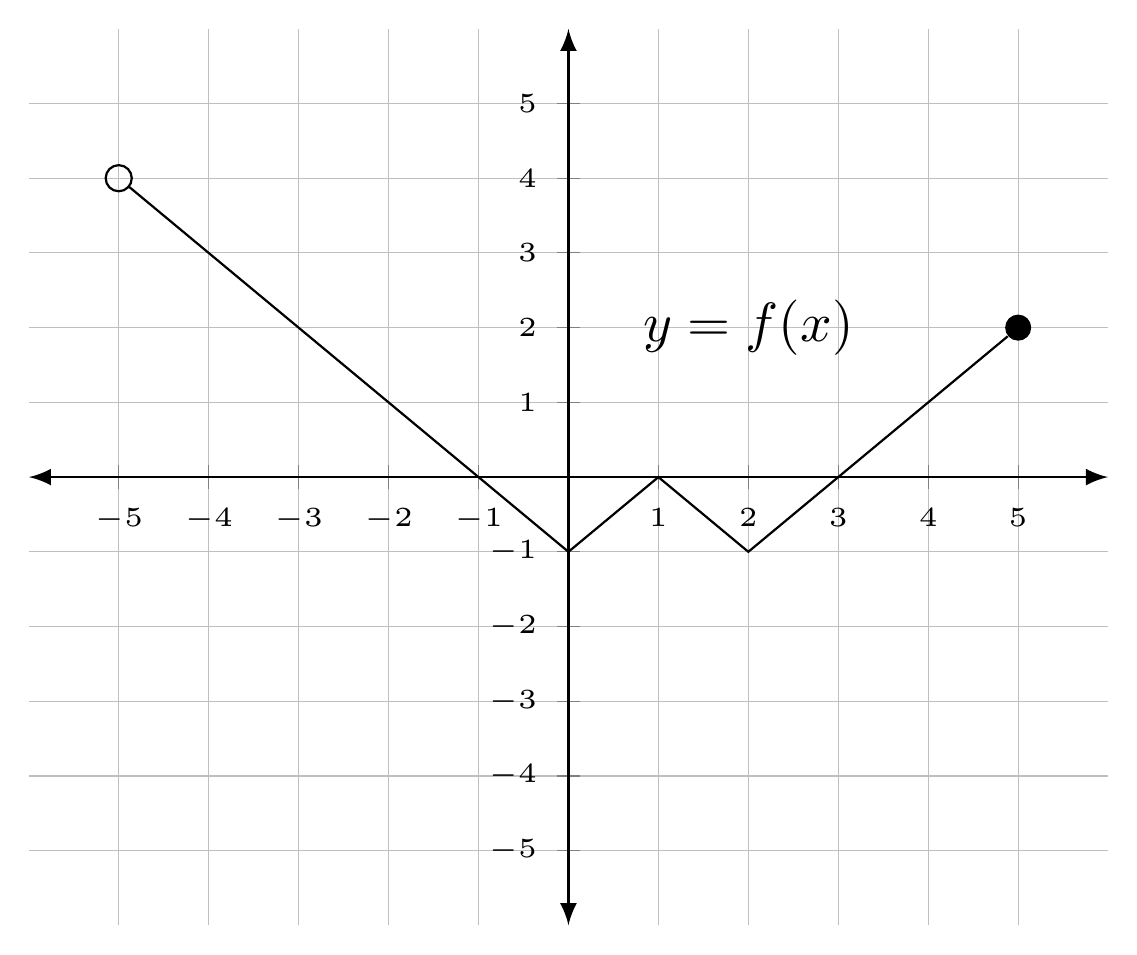
\begin{tikzpicture}[scale=2]
    \begin{axis}[
        xmin=-6,xmax=6,
        ymin=-6,ymax=6,
        grid=both,
        grid style={line width=.1pt, draw=gray!10},
        major grid style={line width=.2pt,draw=gray!50},
        axis lines=middle,
        axis line style={latex-latex},
        xtick={-5,-4,-3,-2,-1,0,1,2,3,4,5},
        ytick={-5,-4,-3,-2,-1,0,1,2,3,4,5},
        ticklabel style={font=\tiny},
      ]
      \node (a) [circle,draw,scale=0.5] at (-5,4) {};
      \node (b) [circle,fill,scale=0.5] at (5,2) {};
      \draw (a) to (0,-1) to (1,0) to (2,-1) to (b);
      \node at (2,2) {$y=f(x)$};
    \end{axis}
  \end{tikzpicture}

  \begin{enumerate}
  \item What is $f(2)$?
    \[f(2)=-1\]
  \item What is the y-intercept?
    \[(0,-1)\]
  \item For what values of $x$ is $f(x)=0$?
    \[x=-1,1,3\]
  \item What is the domain of $f$, in interval notation?
    \[(-5,5]\]
  \item What is the range of $f$, in interval notation?
    \[[-1,4)\]
  \item On what intervals is $f$ increasing?
    \[[0,1]\ \text{and}\ [2,5]\]
  \item On what intervals is $f$ decreasing?
    \[(-5,0]\ \text{and}\ [1,2]\]
  \item What are the local minima (if any)?
    \[(0,-1)\ \text{and}\ (2,-1)\]
  \item What are the local maxima (if any)?
    \[(1,0)\ \text{and}\ (5,2)\]
  \item What is the absolute maximum (if any)?
    \begin{quote}
      none
    \end{quote}
  \end{enumerate}

\item Consider the function: $y=-2\abs{x-2}+3$
  \begin{enumerate}
  \item List the starting standard function and the four transformation steps in the order that they should be
    applied.
    \begin{enumerate}
    \item Basic: \(y=\abs{x}\)
    \item Right 2
    \item Vert Scale 2
    \item Vert Reflect
    \item Up 3
    \end{enumerate}
  \item What are the $x$-intercepts (if any)?
    \begin{gather*}
      0=-2\abs{x-2}+3 \\
      2\abs{x-2}=3 \\
      \abs{x-2}=\frac{3}{2} \\
      x-2=\pm\frac{3}{2} \\
      x=\pm\frac{3}{2}+2 \\
      x=\frac{1}{2},\frac{7}{2} \\
      \\
      \left(\frac{1}{2},0\right)\ \text{and}\ \left(\frac{7}{2},0\right)
    \end{gather*}
  \item What are the $y$-intercepts (if any)?
    \begin{gather*}
      y=-2\abs{0-2}+3=-2(2)+3=-1 \\
      \\
      (0,-1)
    \end{gather*}
  \item What are the local maxima (if any)?
    \[(2,3)\]
  \item What are the local minima (if any)?
    \begin{quote}
      none
    \end{quote}
  \item What is the domain?
    \[\R\]
  \item What is the range?
    \[(-\infty,3]\]
  \item What is the axis of symmetry?
    \[x=2\]
  \item Sketch the graph of the function. Be sure to label all important points.

    \begin{tikzpicture}
      \draw [help lines] (-4,0) -- (4,0);
      \draw [help lines] (0,-4) -- (0,4);
      \draw [dashed] (2,-4) -- (2,4) node [above] {\(x=2\)};
      \draw ({-3/2},-4) -- (2,3) -- ({11/2},-4);
      \filldraw (0,-1) circle [radius=2pt] node [left] {\((0,-1)\)};
      \filldraw ({1/2},0) circle [radius=2pt] node [below right] {\(\left(\frac{1}{2},0\right)\)};
      \filldraw ({7/2},0) circle [radius=2pt] node [below left] {\(\left(\frac{7}{2},0\right)\)};
      \filldraw (2,3) circle [radius=2pt] node [above right] {\((2,3)\)};
    \end{tikzpicture}
  \end{enumerate}
\end{enumerate}

\end{document}
